\documentclass[a4paper, 11pt]{article}
\usepackage{amsmath, amsthm, amsfonts, amssymb, bm, amsopn}
\usepackage{graphicx}
\usepackage{hyperref}

\setlength{\parindent}{0pt}
\setlength{\parskip}{1ex plus 0.5ex minus 0.2ex}

\hypersetup{
    bookmarks=true,         % show bookmarks bar?
    unicode=false,          % non-Latin characters in Acrobat’s bookmarks
    pdftoolbar=false,        % show Acrobat’s toolbar?
    pdfmenubar=true,        % show Acrobat’s menu?
    pdffitwindow=false,     % window fit to page when opened
    pdfstartview={FitH},    % fits the width of the page to the window
    pdftitle={My title},    % title
    pdfauthor={Author},     % author
    pdfsubject={Subject},   % subject of the document
    pdfcreator={Creator},   % creator of the document
    pdfproducer={Producer}, % producer of the document
    pdfkeywords={keywords}, % list of keywords
    pdfnewwindow=true,      % links in new window
    colorlinks=true,       % false: boxed links; true: colored links
    linkcolor=red,          % color of internal links
    citecolor=green,        % color of links to bibliography
    filecolor=magenta,      % color of file links
    urlcolor=cyan           % color of external links
}


\begin{document}
\title{A Comparison of Several Classification Algorithms}
\author{Xinfan Meng \\ \href{mailto:mxf3306@gmail.com}{mxf3306@gmail.com}}
\maketitle

\section{Introduction}

Classification is the task that put data into different categories
based on their characteristics.
For instance, given an book, we can put it into a fiction category
or a science category based on its topic.
Classifier is the computer algorithm that conduct classification task.
There are two types of classification: supervised and unsupervised.
Supervised classifier is the classifier that are given the categories and data in advance, 
from which it can learn how to classify data.
By contrast, unsupervised classifier do not have access to data in advance.


In this report, we are
going to compare the performance of several classification algorithms.
The data we use is the iris dataset.

\section{An Exploration of the Dataset}

Iris dataset is a classic dataset used in classification.
It was first used by Sir Ronald Aylmer Fisher, a renowned statistician.
The dataset contains 50 samples from each of three species of Iris flowers (Iris setosa, Iris virginica and Iris versicolor), 
a genus of 260 species of flowering plants with showy flowers.

First, we will do some exploratory data analysis (EDA) with R and Python.
Let us have a look at the summary of iris dataset.

\begin{verbatim}
import rpy2.robjects as robjects
rsummary = robjects.r("summary(iris)")
print rsummary
\end{verbatim}

This is the output.

\begin{verbatim}
  Sepal.Length    Sepal.Width     Petal.Length    Petal.Width   
 Min.   :4.300   Min.   :2.000   Min.   :1.000   Min.   :0.100  
 1st Qu.:5.100   1st Qu.:2.800   1st Qu.:1.600   1st Qu.:0.300  
 Median :5.800   Median :3.000   Median :4.350   Median :1.300  
 Mean   :5.843   Mean   :3.057   Mean   :3.758   Mean   :1.199  
 3rd Qu.:6.400   3rd Qu.:3.300   3rd Qu.:5.100   3rd Qu.:1.800  
 Max.   :7.900   Max.   :4.400   Max.   :6.900   Max.   :2.500  
       Species  
 setosa    :50  
 versicolor:50  
 virginica :50  
\end{verbatim}

 From the summary, we know each instance in the dataset have Four features: 
sepal length sepal width, petal length and petal width
(species is not considered a feature since that is what we would like to predict).

Then we draw a scatter plot of the dataset.
\begin{verbatim}
pairs(iris, main="Iris Data (red=setosa,green=versicolor,blue=virginica)", pch=21,
  bg=c("red","green3","blue")[unclass(iris$Species)])
\end{verbatim}

\begin{figure}[htbp]
  \begin{center}
    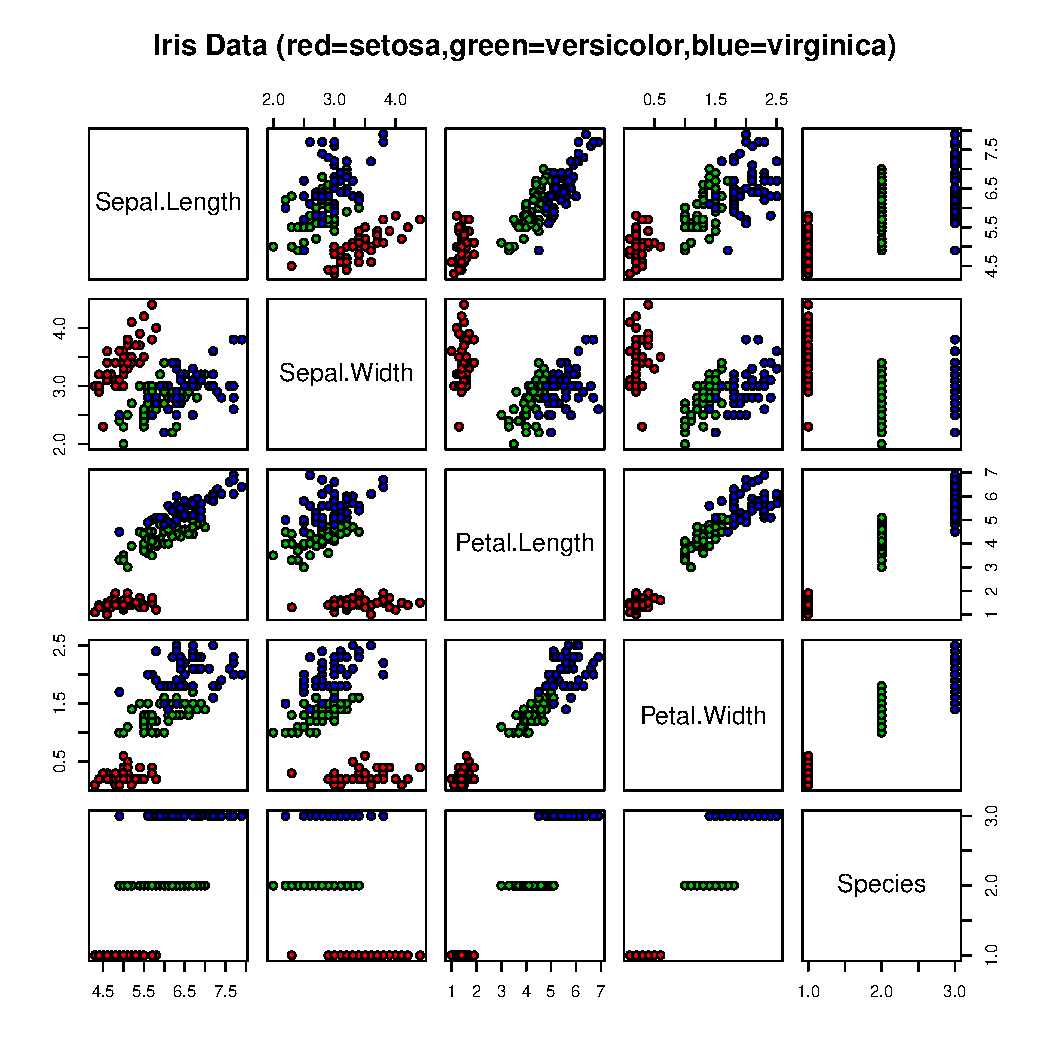
\includegraphics[width=0.75\linewidth]{1.pdf}
  \end{center}
  \caption{scatter plot of iris dataset}
  \label{fig:iris}
\end{figure}
 
From figure \ref{fig:iris}, we can see that most features have considerable power in 
discriminating species.


\section{Experiments}
In the following experiments, we will
evaluate three algorithms on the iris dataset.
These three algorithms are: Support Vector Machine (SVM),
nearest neighbors and logistic regression.
These algorithms have very different characteristics.
SVM is a maximum-margin linear classifier.
Logistic regression is a probabilistic linear classifier.
Nearest neighbors is a non-parametric non-linear classifer.
The detailed description of each algorithm can be found in \cite{prml}.

We use the following script to compute each algorithm's accuracy rspectively. 
\begin{verbatim}
from scikits.learn import datasets
from scikits.learn.cross_val import StratifiedKFold
from scikits.learn import svm
from scikits.learn.linear_model import LogisticRegression
from scikits.learn import neighbors
from rpy2 import robjects
from rpy2.robjects import FloatVector as rfloat
import numpy as np

iris = datasets.load_iris()

def test_algorithm(algorithm, results, train_data, train_target, test_data):
    algorithm.fit(train_data, train_target)
    y_pred = algorithm.predict(test_data)
    results.append(precision(y_pred))

def precision(y_pred):
    prec = sum(y_pred == test_target)
    return float(prec) / len(test_target)

svmclf = svm.SVC()
logisticclf = LogisticRegression()
nnclf= neighbors.Neighbors()
svmli = []
logli = []
nnli = []

cv = StratifiedKFold(iris.target, 20)
for train_index, test_index in cv:
    train_data = iris.data[train_index]
    train_target = iris.target[train_index]
    test_data = iris.data[test_index]
    test_target = iris.target[test_index]

    #svm
    test_algorithm(svmclf, svmli, train_data, train_target, test_data)

    #logistic regression
    test_algorithm(logisticclf, logli, train_data, train_target, test_data)
    
    #NN
    test_algorithm(nnclf, nnli, train_data, train_target, test_data)


print "Precison of each algortihm:"
print "SVM:", np.average(svmli)
print "logistic regression:", np.average(logli)
print "nearest neighbors:", np.average(nnli)
print
\end{verbatim}

Then we use paired t test to comapre their accuracies \cite{mitchell} \cite{r}.

\begin{verbatim}
rttest = robjects.r["t.test"]
print "Paired t-test between algorithms:"
print "SVM vs logistic regression",
tt =  rttest(rfloat(svmli), rfloat(logli), paired=True)
print "p-value", tt.rx('p.value')[0][0]
print "SVM vs nearest neighbors",
tt = rttest(rfloat(svmli), rfloat(nnli), paired=True)
print "p-value", tt.rx('p.value')[0][0]
print "nearest neighbors vs logistic regression",
tt = rttest(rfloat(logli), rfloat(nnli), paired=True)
print "p-value", tt.rx('p.value')[0][0]
\end{verbatim}

The following is the output.

\begin{verbatim}
Precison of each algortihm:
SVM: 0.927777777778
logistic regression: 0.941666666667
nearest neighbors: 0.958333333333

Paired t-test between algorithms:
SVM vs logistic regression p-value 0.715682107694
SVM vs nearest neighbors p-value 0.185647078924
nearest neighbors vs logistic regression p-value 0.540884257545
\end{verbatim}

Clearly, every p-value is less than $0.95$, so the 
difference is statistically significant.
Based on the above analysis, 
we conclude that nearest neighbors is the best and
SVM is the worst on the iris dataset.

\section{Conclusion}

In this report, we report three classic algorithms on a classic dataset.
The experiments rank nearest neighbor classifier as the best out-of-box 
classifier.
In later study, we will try some feature selection algorithms
and hyper-parameter tuning techniques to further investigate each algorithm.

\begin{thebibliography}{99}
  \bibitem{prml} Christopher M. Bishop, Pattern Recognitio and Machine Learning.
  \bibitem{r} Xue yi Chen Liping, R stattistical modelling and R software (in Chinese).
  \bibitem{mitchell} Tom M. Mitchell, Machine learning.
\end{thebibliography}

\end{document}
